\subsection{Połączenie mostkowe}


\subsubsection{Wstęp}

Połączenie mostkowe działa identycznie jak przełącznik (\emph{switch}) w sieci.
Mostek i przerzutnik są w stanie połączyć wiele fizycznych podsieci na poziomie
warstwy łącza modelu OSI. Pozwala to uniknąć konfiguracji dodatkowych puli
adresów IP.

Zasada działania mostka i przełącznika są podobne. Do każdego portu mostka
podłączona jest ina podsieć. W miarę upływu czasu i ruchu na mostku, zapełniana
jest tablica filtrująca. Tablica mapuje adresy MAC maszyn na porty, czyli
efektywnie na podsieci, do których maszyny te są podłączone
\cite{mostek:stevens-wstep}. Przy pełnej tablicy filtrującej, mostek przepuszcza
jedynie ramki wysyłanie pomiędzy maszynami z różnych podsieci. Ruch lokalny dla
podsieci jest blokowany przez mostek. Gdy mostek nie jest w stanie
przyporządkować adresu MAC do jednej z podsieci, wtedy dana ramka jest rozsyłana
do wszystkich podłączonych podsieci oprócz podsieci nadawcy. Przy otrzymaniu
odpowiedzi, dodawany jest nowy wpis w tablicy.

Różnica między przełącznikiem a mostkiem jest w możliwości konfiguracji mostków.
Mostki pozwalają na pracę w kilku trybach pracy `nauki' nowych adresów MAC.
Swobodę konfiguracji można wykorzystać przy rozdzielaniu sieci VLAN lub stworzyć
prostą zaporę sieciową. Z kolei przełączniki, dzięki prostszym zasadom pracy,
pozwalają na wydajniejszą pracę.


\subsubsection{Wykonanie ćwiczenia}

W ramach ćwiczenia, stworzono mostek w popularnym scenariuszu połączenia małej
sieci WLAN do sieci laboratorium. Skonfigurowano połączenie \wifi{} w trybie
ad\dywiz hoc pomiędzy maszynami \kp{} i \ks. Na połączeniu ręcznie ustawiono
sieć o adresie \texttt{10.0.0.0/24} i przypisano maszynom odpowiednio adresy
\texttt{10.0.0.5} i \texttt{10.0.0.7}. Schemat nr
\ref{fig:mostek:schemat_po_konfiguracji} przedstawia wykorzystane połączenia.

\begin{figure}[h!]
  \centering
  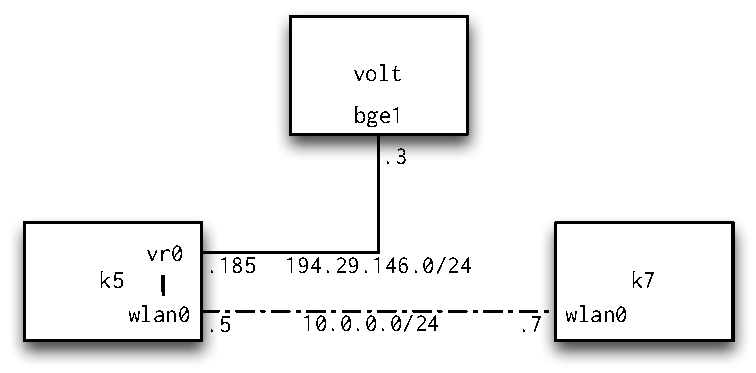
\includegraphics[width=11cm]{figury/mostek/schemat-po-konfiguracji.pdf}
  \caption{Schemat dwóch sieci połączonych mostkiem.}
  \label{fig:mostek:schemat_po_konfiguracji}
\end{figure}

Na maszynie \kp{} ustawiono dwuportowy mostek na interfejsach \texttt{vr0} i
\texttt{wlan0}, z włączonym protokołem STP dla obydwu portów.

\begin{lstlisting}
k5% sudo ifconfig bridge create
bridge0
k5% ifconfig bridge0
bridge0: flags=8802<BROADCAST,SIMPLEX,MULTICAST> metric 0 mtu 1500
    ether 02:7d:1d:ad:cc:00
    id 00:00:00:00:00:00 priority 32768 hellotime 2 fwddelay 15
    maxage 20 holdcnt 6 proto rstp maxaddr 2000 timeout 1200
    root id 00:00:00:00:00:00 priority 0 ifcost 0 port 0
k5% sudo ifconfig bridge0 \
        addm vr0 stp vr0 \
        addm wlan0 stp wlan0
k5% ifconfig bridge0
bridge0: flags=8802<BROADCAST,SIMPLEX,MULTICAST> metric 0 mtu 1500
    ether 02:7d:1d:ad:cc:00
    id 00:0f:cb:ff:13:a7 priority 32768 hellotime 2 fwddelay 15
    maxage 20 holdcnt 6 proto rstp maxaddr 2000 timeout 1200
    root id 00:0f:cb:ff:13:a7 priority 32768 ifcost 0 port 0
    member: wlan0 flags=147<LEARNING,DISCOVER,STP,AUTOEDGE,AUTOPTP>
            ifmaxaddr 0 port 5 priority 128 path cost 370370 proto rstp
            role designated state discarding
    member: vr0 flags=1c7<LEARNING,DISCOVER,STP,AUTOEDGE,PTP,AUTOPTP>
            ifmaxaddr 0 port 1 priority 128 path cost 200000 proto rstp
            role designated state discarding
\end{lstlisting}

Następnie włączono nasłuchiwanie pakietów na interfejsie \texttt{wlan0} maszyny
\ks{}. Ruch z sieci laboratorium pojawił się dopiero w chwili włączenia mostku
na maszynie \kp.

\begin{lstlisting}
k5% sudo ifconfig bridge0 up

k7% sudo tcpdump -i wlan0
tcpdump: verbose output suppressed, use -v or -vv for full protocol decode
listening on wlan0, link-type EN10MB (Ethernet), capture size 65535 bytes
01:28:57.118321 ARP, Request who-has 192.168.123.118 tell 192.168.146.3, length 46
01:28:57.609479 ARP, Request who-has 192.168.2.70 tell 192.168.2.70, length 46
01:28:58.354328 STP 802.1w, Rapid STP, Flags [Learn, Forward], bridge-id 8000.K5-W.8005, length 36
...
\end{lstlisting}

Przy włączonym mostku tablica filtrująca rozszerzała się o nowe wpisy.
Przyjrzyjmy się dwóm wybranym wpisom. Pierwszy przypisuje adres interfejsu
\texttt{bge1} maszyny \volt{}, do interfejsu \texttt{vr0} mostka. Drugi rząd
informuje o interfejsie \texttt{wlan0} maszyny \texttt{k7}, który jest dostępny
poprzez interfejs \texttt{wlan0} mostka.

\begin{lstlisting}
k5% sudo ifconfig bridge0 addr
00:e0:81:65:37:d4 Vlan1 vr0 1199 flags=0<>    # adres MAC bge1 na volt
00:0e:2e:c4:2f:e7 Vlan1 wlan0 1198 flags=0<>  # adres MAC wlan0 na k7
\end{lstlisting}

Obecność tych wpisów potwierdza poprawność konfiguracji mostka, zgodnie ze
schematem z rysunku \ref{fig:mostek:schemat_po_konfiguracji}.


\subsubsection{Komentarz}

Utworzenie mostka w warunkach domowych pomiędzy wirtualną siecią \eth{} a
siecią \wifi, okazało się nieco problematyczne.

Próbując ustanowić mostek między interfejsem \eth{} maszyny wirtualnej a
interfejsem fizycznej karty bezprzewodowej przepływ ruchu nie był możliwy ze
względu na różne wartości MTU tych interfejsów. W przypadku, gdy użytkownik nie
ma możliwości edycji wartości MTU, ustanowienie mostka jest niemożliwe.

Zauważono też, że pakiety pochodzące z interfejsu fizycznej karty
bezprzewodowej, są odrzucane przez niektóre urządzenia \wifi. Logi wykazały, że
pakiety zostały uznane za próbe oszustwa w ramach ataku \emph{MAC spoofing}. W
odrzuconych pakietach adres MAC nadawcy różnił się od spodziewanego adresu MAC
fizycznej karty sieciowej. Odrzucony adres MAC był adresem MAC interfejsu zza
mostka. Jest to fałszywy alarm, jednak odróżnienie takiego scenariusza od
faktycznego ataku jest nietrywialne.
